\documentclass[submit]{harvardml}

\course{CS181-S24}
\assignment{Assignment \#6}
\duedate{11:59PM EST, April 26 2024}
\newcommand{\attr}[1]{\textsf{#1}}
\usepackage[OT1]{fontenc}
\usepackage{float}
\usepackage[colorlinks,citecolor=blue,urlcolor=blue]{hyperref}
\usepackage[pdftex]{graphicx}
\usepackage{subfig}
\usepackage{fullpage}
\usepackage{amsmath}
\usepackage{amssymb}
\usepackage{color}
\usepackage{todonotes}
\usepackage{listings}
\usepackage{common}
\usepackage{bm}
\usepackage{enumitem}
\usepackage{tikz}
\usepackage{xifthen}
\usepackage{soul}
\usepackage{framed}

\usepackage[mmddyyyy,hhmmss]{datetime}

\definecolor{verbgray}{gray}{0.9}

\lstnewenvironment{csv}{
  \lstset{backgroundcolor=\color{verbgray},
  frame=single,
  framerule=0pt,
  basicstyle=\ttfamily,
  columns=fullflexible}}{}

\newcommand{\mueps}{\mu_{\epsilon}}
\newcommand{\sigeps}{\sigma_{\epsilon}}
\newcommand{\mugam}{\mu_{\gamma}}
\newcommand{\siggam}{\sigma_{\gamma}}
\newcommand{\muzp}{\mu_{p}}
\newcommand{\sigzp}{\sigma_{p}}
\newcommand{\gauss}[3]{\frac{1}{2\pi#3}e^{-\frac{(#1-#2)^2}{2#3}}}

%%%%%%%%%%%%%%%%%%%%%%%%%%%%%%%%%%
%% Solution environment
\newenvironment{solution}
  {\color{blue}\section*{Solution}}
{}
%%%%%%%%%%%%%%%%%%%%%%%%%%%%%%%%%%

\begin{document}
\begin{center}
{\Large Homework 6: Inference in Graphical Models, MDPs}\\
\end{center}

\subsection*{Introduction}

In this assignment, you will practice inference in graphical models as
well as MDPs/RL.

\subsection*{Resources and Submission Instructions}

For readings, we recommend \href{http://incompleteideas.net/book/the-book-2nd.html}{Sutton and Barto 2018, Reinforcement Learning: An Introduction}, \href{https://harvard-ml-courses.github.io/cs181-web/}{CS181  Lecture Notes}, and Section 10 and 11 Notes.

Please type your solutions after the corresponding problems using this
\LaTeX\ template, and start each problem on a new page.

Please submit the \textbf{writeup PDF to the Gradescope assignment `HW6'}. Remember to assign pages for each question.

Please submit your \textbf{\LaTeX\ file and code files to the Gradescope assignment `HW6 - Supplemental'}. 

You can use a \textbf{maximum of 2 late days} on this assignment.  Late days will be counted based on the latest of your submissions. 
\\

\newpage

\begin{problem}[Hidden Markov Models, 15 pts]
In this problem, you will be working with one-dimensional Kalman filters, which are \textit{continuous-state} Hidden Markov Models. Let $z_0, z_1, \cdots , z_t$ be the hidden states of the system and $x_0, x_1, \cdots, x_t$ be the observations produced. Then, state transitions and emissions of observations work as follows:
  \begin{eqnarray*}
    z_{t+1} &= z_{t} + \epsilon_{t} \\
    x_{t} & = z_{t} + \gamma_{t}
  \end{eqnarray*}
 where $\epsilon_t \sim N(0,\sigeps^2)$ and $\gamma_t \sim N(0,\siggam^2)$. The value of the first hidden state follows the distribution $z_0 \sim N(\muzp,\sigzp^2)$.

\begin{enumerate}
  \item Draw the graphical model corresponding to the one-dimensional Kalman filter.
  \item In this part we will walk through the derivation of the conditional distribution of $z_t|(x_0, \cdots, x_{t})$.
  \begin{enumerate}
      \item How does the quantity $p(z_t| x_0, \cdots, x_{t})$ relate to $\alpha_t(z_t)$ and $\beta_t(z_t)$ from the forward-backward algorithm for HMMs?  What is the operation we are performing called?
      \item The above quantity $p(z_t|x_0, \cdots, x_t)$ is the PDF for a Normal distribution with mean $\mu_t$ and variance $\sigma_t^2$. We start our derivation of $\mu_t$ and $\sigma_t^2$ by writing:
      \begin{align*}
          p(z_t|x_0, \cdots, x_t) \propto p(x_t|z_t)p(z_t|x_0, \cdots x_{t-1})
      \end{align*}
      What is $p(x_t|z_t)$ equal to?
      \item Suppose we are given the mean and variance of the distribution $z_{t-1}|(x_0, \cdots, x_{t-1})$ as $\mu_{t-1}$, $\sigma^2_{t-1}$. What is $p(z_t|x_0, \cdots x_{t-1})$ equal to? 
      
      \textbf{Hint 1}: Start by marginalizing out over $z_{t-1}$.
      
      \textbf{Hint 2}: You may cite the fact that 
      \[\int N(y-x ; \mu_a, \sigma^2_a)N(x ; \mu_b, \sigma^2_b)dx = N(y ; (\mu_a + \mu_b), (\sigma^2_a + \sigma^2_b))\]
      \item Combine your answers from parts (b) and (c) to get a final expression for $p(z_t|x_0, \cdots, x_t)$. Report the mean $\mu_t$ and variance $\sigma_t^2$ of this Normal.
      
      \textbf{Hint 1}: Rewrite $N(x_t; z_t, \siggam^2)$ as $N(z_t; x_t, \siggam^2)$.
      
      \textbf{Hint 2}: You may cite the fact that 
      \[N(x; \mu_a, \sigma^2_a)N(x; \mu_b, \sigma^2_b) = N\left(x; \frac{\sigma^2_b}{\sigma^2_a+\sigma^2_b}\mu_a + \frac{\sigma^2_a}{\sigma^2_a+\sigma^2_b}\mu_b, \ \left(\frac{1}{\sigma^2_a} + \frac{1}{\sigma^2_b}\right)^{-1}\right)\]
  \end{enumerate}
  \item Interpret $\mu_t$ in terms of how it combines observations from the past with the current observation. 
\end{enumerate}
\end{problem}


\begin{solution}
	Your solution here.
\end{solution}

\newpage

\begin{problem}[Policy and Value Iteration, 15 pts]

You have a robot that you wish to collect two parts in an environment
and bring them to a goal location.  There are also parts of the
environment that you wish the robot avoid to reduce wear on the floor.

Eventually, you settle on the following way to model the environment
as a Gridworld.  The ``states'' in Gridworld are represented by
locations in a two-dimensional space.  Here we show each state and its
reward:

\begin{center}
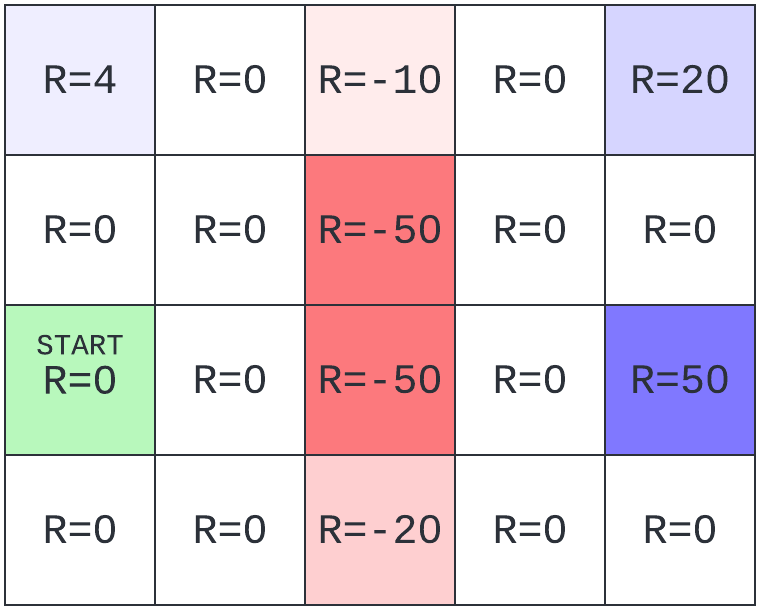
\includegraphics[width=3in]{images/gridworld.png}
\end{center}

The set of actions is \{N, S, E, W\}, which corresponds to moving north (up), south (down), east (right), and west (left) on the grid. Taking an action in Gridworld does not always succeed with probability
$1$; instead the agent has probability $0.1$ of ``slipping'' into a
state on either side, but not backwards.  For example, if the agent tries to move right from START, it succeeds with probability 0.8, but the agent may end up moving up or down with probability 0.1 each. Also, the agent cannot move off the edge of the grid, so moving left from START will keep the agent in the same state with probability 0.8, but also may slip up or down with probability 0.1 each. Lastly, the agent has no chance of slipping off the grid - so moving up from START results in a 0.9 chance of success with a 0.1 chance of moving right.

Also, the agent does not receive the reward of a state immediately upon entry, but instead only after it takes an action at that state. For example, if the agent moves right four times (deterministically, with no chance of slipping) the rewards would be +0, +0, -50, +0, and the agent would reside in the +50 state. Regardless of what action the agent takes here, the next reward would be +50.

In this problem, you will first implement policy and value iteration in this setting and discuss the policies that you find.  Next, you will interrogate whether this approach to modeling the original problem was appropriate.

\end{problem}
\newpage

\begin{framed}
\textbf{Problem 2} (cont.)\\

Your job is to implement the following three methods in file \texttt{homework6.ipynb}. Please use the provided helper functions \texttt{get\_reward} and \texttt{get\_transition\_prob} to implement your solution. \emph{Do not use any outside code.  (You may still collaborate with others according to the standard collaboration policy in the syllabus.)}  

\textbf{Important: } The state space is represented using integers, which range from 0 (the top left) to 19 (the bottom right). Therefore both the policy \texttt{pi} and the value function \texttt{V} are 1-dimensional arrays of length \texttt{num\_states = 20}. Your policy and value iteration methods should only implement one update step of the iteration - they will be repeatedly called by the provided \texttt{learn\_strategy} method to learn and display the optimal policy. You can change the number of iterations that your code is run and displayed by changing the $\texttt{max\_iter}$ and $\texttt{print\_every}$ parameters of the $\texttt{learn\_strategy}$ function calls at the end of the code.

Note that we are doing infinite-horizon planning to maximize the expected reward of the traveling agent. For parts 1-3, set discount factor $\gamma = 0.7$.

\begin{itemize}
    \item[1a.]  Implement function \texttt{policy\_evaluation}.  Your
      solution should learn value function $V$, either using a closed-form expression or iteratively using
      convergence tolerance $\texttt{theta = 0.0001}$ (i.e., if
      $V^{(t)}$ represents $V$ on the $t$-th iteration of your policy
      evaluation procedure, then if $|V^{(t + 1)}[s] - V^{(t)}[s]|
      \leq \theta$ for all $s$, then terminate and return $V^{(t + 1)}$.)
      % FDV: Check for discrepancies between the staff code and the tolerance listed here -- resolved
    \item[1b.] Implement function \texttt{update\_policy\_iteration} to update the policy \texttt{pi} given a value function \texttt{V} using \textbf{one step} of policy iteration.
    
    \item[1c.] Set \texttt{max\_iter = 4}, \texttt{print\_every = 1} to show the learned value function and the associated policy for the first 4 policy iterations. Do not modify the plotting code. Please fit all 4 plots onto one page of your writeup.
    
    \item [1d.] Set \texttt{ct = 0.01} and increase \texttt{max\_iter} such that the algorithm converges. Include a plot of the final learned value function and policy. How many iterations does it take to converge? Now try \texttt{ct = 0.001} and \texttt{ct = 0.0001}. How does this affect the number of iterations until convergence?
      
    \item [2a.] Implement function
      \texttt{update\_value\_iteration}, which performs \textbf{one step} of value iteration to update \texttt{V}, \texttt{pi}.
      
    \item [2b.] Set \texttt{max\_iter = 4}, \texttt{print\_every = 1} to show the learned value function and the associated policy for the first 4 value iterations. Do not modify the plotting code. Please fit all 4 plots onto one page of your writeup.
    
    \item [2c.] Set \texttt{ct = 0.01} and increase \texttt{max\_iter} such that the algorithm converges. Include a plot of the final learned value function and policy. How many iterations does it take to converge? Now try \texttt{ct = 0.001} and \texttt{ct = 0.0001}. How does this affect the number of iterations until convergence?
    
    \item[3.] Compare and contrast the number of iterations, time per iteration, and overall runtime between policy iteration and value iteration. What do you notice?
    
    \item[4.] Plot the learned policy with each of $\gamma \in (0.6,0.7,0.8,0.9)$. Include all 4 plots in your writeup. Describe what you see and provide explanations for the differences in the observed policies. Also discuss the effect of gamma on the runtime for both policy and value iteration.
    
    \item[5.] Now suppose that the game ends at any state with a positive reward, i.e. it immediately transitions you to a new state with zero reward that you cannot transition away from. What do you expect the optimal policy to look like, as a function of gamma? Numerical answers are not required, intuition is sufficient.
 
\end{itemize}
\end{framed}

\newpage 

\begin{framed}
\textbf{Problem 2} (cont.)\\

Now you will interrogate your solution in terms of its applicability
for the intended task of picking up two objects and bringing them to a
goal location.

\begin{itemize}

  \item[6.] In this problem, we came up with a model for the problem,
    solved it, and then we had a policy to use on the real robot.  An
    alternative could have been to use RL on the robot to identify a
    policy that achieved your objective.  What is the value of the
    approach we took?  What are some limitations (in general)? 


  \item[7.] Do any of the policies learned actually accomplish the task
    that you desired?  What modeling shortcuts were made that result
    in some policies matching your true objective and some not?

    
  \item[8.] Describe at least three modeling choices that were made in
    turning your original goal into this abstract problem, and
    potential implications of those choices.
 

\end{itemize}

\end{framed}

\begin{solution}
	Your solution here.
\end{solution}


\begin{problem}[Reinforcement Learning, 20 pts]
  In 2013, the mobile game \emph{Flappy Bird} took the world by storm. You'll be developing a Q-learning agent to play a similar game, \emph{Swingy Monkey} (See Figure~\ref{fig:swingy}).  In this game, you control a monkey that is trying to swing on vines and avoid tree trunks.  You can either make him jump to a new vine, or have him swing down on the vine he's currently holding.  You get points for successfully passing tree trunks without hitting them, falling off the bottom of the screen, or jumping off the top.  There are some sources of randomness: the monkey's jumps are sometimes higher than others, the gaps in the trees vary vertically, the gravity varies from game to game, and the distances between the trees are different.  You can play the game directly by pushing a key on the keyboard to make the monkey jump.  However, your objective is to build an agent that \emph{learns} to play on its own. 
  
   You will need to install the \verb|pygame| module
  (\url{http://www.pygame.org/wiki/GettingStarted}).
  

\textbf{Task:}
Your task is to use Q-learning to find a policy for the monkey that can navigate the trees.  The \verb|homework6_soln.ipynb| file contains starter code for setting up your learner that interacts with the game. This is the \textbf{only code file} you need to modify. At the beginning of the code, you will import the \verb|SwingyMonkey| class, which is the implementation of the game that has already been completed for you. Note that by default we have you import this class from the file \verb|SwingyMonkeyNoAnimation.py|, which allows you to speed up testing. To actually see the game animation, you can instead import from \verb|SwingyMonkey.py|. Additionally, we provide a video of the staff Q-Learner playing the game at \url{https://youtu.be/xRD6xBQbauw}.  It figures out a reasonable policy in a few iterations.
You'll be responsible for implementing the Python function  \verb|action_callback|. The action callback will take in a dictionary that describes the current state of the game and return an action for the next time step.  This will be a binary action, where 0 means to swing downward and 1 means to jump up.  The dictionary you get for the state looks like this:
\begin{csv}
{ 'score': <current score>,
  'tree': { 'dist': <pixels to next tree trunk>,
            'top':  <height of top of tree trunk gap>,
            'bot':  <height of bottom of tree trunk gap> },
  'monkey': { 'vel': <current monkey y-axis speed>,
              'top': <height of top of monkey>,
              'bot': <height of bottom of monkey> }}
\end{csv}
All of the units here (except score) will be in screen pixels. Figure~\ref{fig:swingy-ann} shows these graphically. 
Note that since the state space is very large (effectively continuous), the monkey's relative position needs to be discretized into bins. The pre-defined function \verb|discretize_state| does this for you.

\textbf{Requirements}
\\
\textit{Code}: First, you should implement Q-learning with an
$\epsilon$-greedy policy yourself. You can increase the performance by
trying out different parameters for the learning rate $\alpha$,
discount rate $\gamma$, and exploration rate $\epsilon$. \emph{Do not use outside RL code for this assignment.} Second, you should use a method of your choice to further improve the performance. This could be inferring gravity at each epoch (the gravity varies from game to game), updating the reward function, trying decaying epsilon greedy functions, changing the features in the state space, and more. One of our staff solutions got scores over 800 before the 100th epoch, but you are only expected to reach scores over 50 before the 100th epoch. {\bf Make sure to turn in your code!} \\\\

\textit{Evaluation}: In 1-2 paragraphs, explain how your agent performed and what decisions you made and why. Make sure to provide evidence where necessary to explain your decisions. You must include in your write up at least one plot or table that details the performances of parameters tried (i.e. plots of score vs. epoch number for different parameters). \\\\

\textit{Note}: Note that you can simply discretize the state and action spaces and run the Q-learning algorithm. There is no need to use complex models such as neural networks to solve this problem, but you may do so as a fun exercise.

\end{problem}
\begin{figure}[H]
    \centering%
    \subfloat[SwingyMonkey Screenshot]{%
        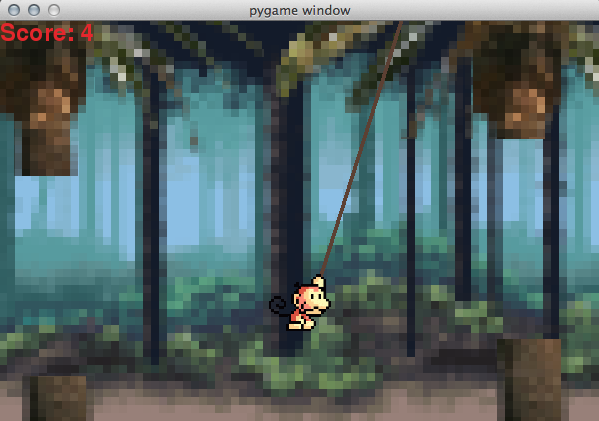
\includegraphics[width=0.48\textwidth]{images/swingy}
        \label{fig:swingy}
    }\hfill
    \subfloat[SwingyMonkey State]{%
        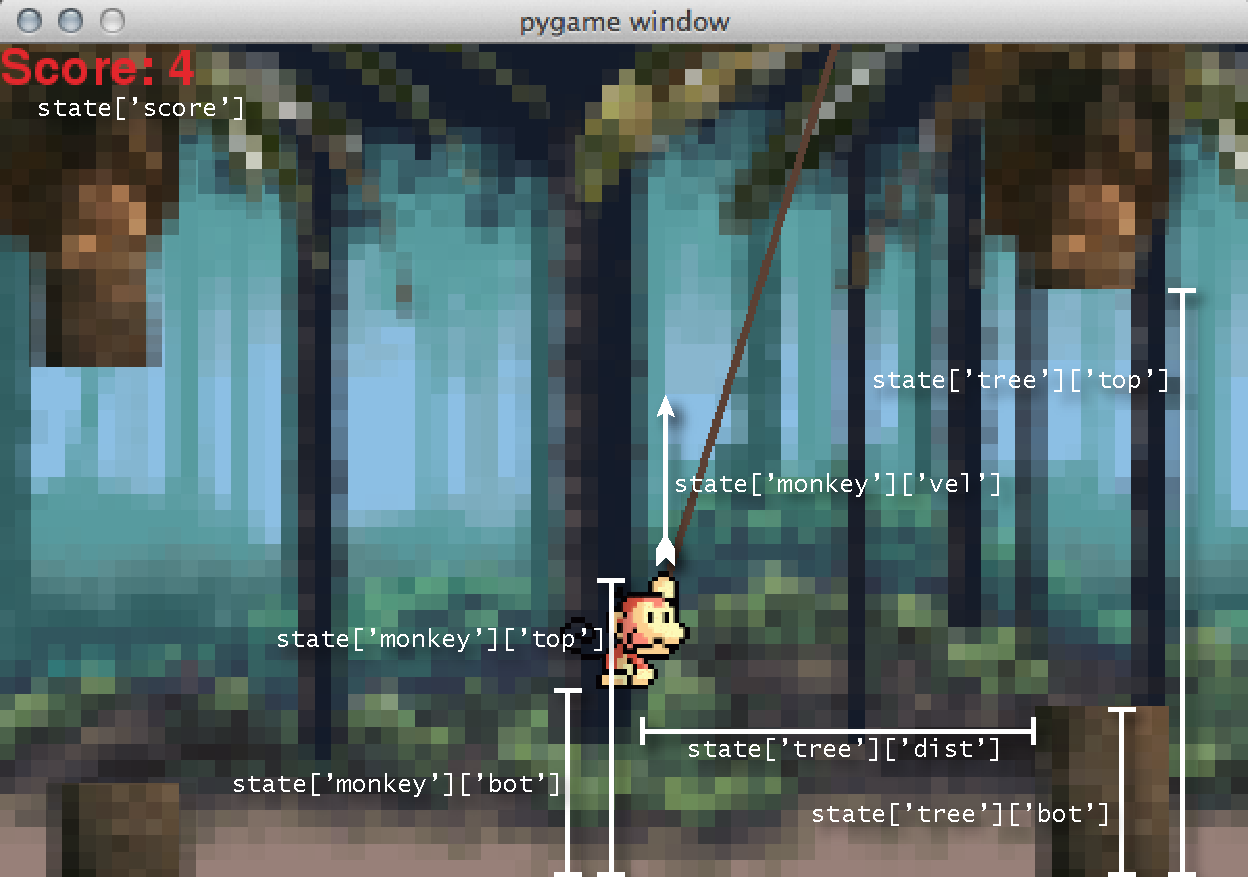
\includegraphics[width=0.48\textwidth]{images/swingy-ann}
        \label{fig:swingy-ann}
    }
    \caption{(a) Screenshot of the Swingy Monkey game.  (b) Interpretations of various pieces of the state dictionary.}
\end{figure}
    

\begin{solution}
	Your solution here.
\end{solution}

\newpage
%%%%%%%%%%%%%%%%%%%%%%%%%%%%%%%%%%%%%%%%%%%%%
% Name and Calibration
%%%%%%%%%%%%%%%%%%%%%%%%%%%%%%%%%%%%%%%%%%%%%
\newpage
\subsection*{Name}
\subsection*{Collaborators and Resources}
Whom did you work with, and did you use any resources beyond cs181-textbook and your notes?

\end{document}
